\documentclass{article}
\usepackage[utf8]{inputenc}
\usepackage{kotex} % 한국어를 가능하도록 해주는 패키지 입니다. 
\usepackage[left=2.5cm,right=2.5cm,top=3cm,bottom=3cm,a4paper]{geometry} % 페이지 레이아웃 설정입니다. 
\usepackage{listings}  % 소스코드 작성에 필요한 패키지 입니다. 헤더파일이랑 비슷한 개념입니다. 
% 소스코드는 \begin{lstlisting} 이 사이에 써야됩니다. \end{lstlisting}
% 이건 주석입니다. 
% // 이건 개행입니다. 
% \indent 이건 들여쓰기입니다. 
% 논문 링크는 references.bib에서 수정한 후에 
% 이 파일로 돌아와서 해당 부분에 \citep[이름] 코드를 붙여야합니다. 
% 사진의 경우 import 후 30번째 줄을 참고하시면 됩니다. 
\usepackage{color} % 컬러 패키지 입니다 

\usepackage{hyperref} \hypersetup{ 
colorlinks=true, linkcolor=blue, filecolor=magenta, urlcolor=cyan, }

\usepackage{ textcomp }


\title{Darknet YOLO API}
\author{이대경, 김한섭, 강일송 }
\date{2017학년도 2학기 오픈소스 Team Project}

\usepackage{natbib}
\usepackage{graphicx}

\begin{document}

\maketitle

\section{You Only Look Once}

\indent YOLO시스템은 최첨단 실시간 물체 감지 시스템이다.
기존의 탐지시스템은 Repurpose classifiers 혹은 Localizers를 사용하여 탐지를 수행하였습니다. 이 방법은 모델의 여러 위치에 격자 이미지를 적용하는 방식이며 격자 중 높은 일치도를 보인 물체를 탐지합니다. 하지만 YOLO는 하나의 신경망을 전체 이미지에 적용하는 완전히 다른 방식을 사용합니다. 이 신경망은 이미지를 여러 영역으로 분할하고 각 영역에 대한 바운딩 영역과 가중치로 사용될 일치 확률을 예측하여 줍니다.

\begin{figure}[h!]
\centering
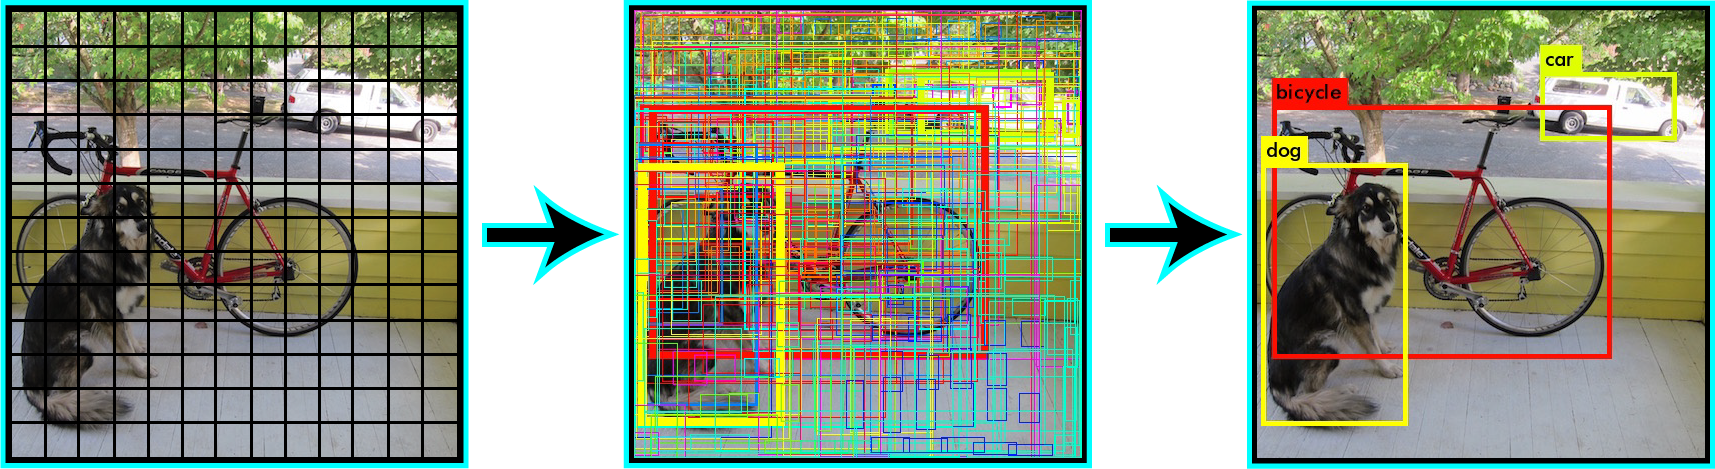
\includegraphics[scale=0.2]{model2.png}
\caption{탐지과정}
\label{fig:detect}
\end{figure}

YOLO 시스템은 분류 기반의 시스템에 비해 몇 가지 장점을 가지고 있다.
그 중 하나는 테스트 시간 동안 전체 이미지를 보고 예측된 정보를 이미지에 텍스트로 알려줍니다. 또한 수천개의 단일 이미지가 필요한 R-CNN 과는 달리 단일 네트워크만으로 평가하고 예측이 가능합니다. 이로 인해 R-CNN보다는 1000배 이상 빠르며 Fast R-CNN보다는 100배 빠릅니다. 전체 시스템에 대한 자세한 내용은 해당 논문\citep{YOLO9000} 을 참고하시기 바랍니다.


\section{탐지기법 실습}

\indent 사전 훈련 된 모델을 사용하여 YOLO 시스템으로 물체를 탐지 하는 방법을 설명합니다. 
Darknet을 아직 설치 하지 않았다면 먼저 설치 해야합니다. \\
이제부터 아래의 명령어를 실행하시기바랍니다.\\
\begin{lstlisting}.
 git clone https://github.com/pjreddie/darknet
 cd darknet 
 make
\end{lstlisting}
실행 후 cfg/ 서브디렉토리에 YOLO에 대한 설정 파일이 존재합니다. 
\\사전 훈련된 가중치를 다운로드한 뒤
\begin{lstlisting}
 wget https://pjreddie.com/media/files/yolo.wegith
\end{lstlisting}
다음을 실행하시기 바랍니다.
\begin{lstlisting}
/darknet detect cfg/yolo.cfg yolo.weights data/dog.jpg 
\end{lstlisting}
여기까지 실행하시면 다음과 같은 출력이 표시됩니다.\\
\begin{lstlisting}
   .layer filters size input output 
   0 conv 32 3 x 3 / 1 416 x 416 x 3 -> 416 x 416 x 32 
   1 max 2 x 2 / 2 416 x 416 x 32 -> 208 x 208 x 32 
   ....... 
   29 conv 425 1 x 1 / 1 13 x 13 x1024 -> 13 x 13 x 425 
   30 detection 
   Loading weights from yolo.weights...Done! 
   data/dog.jpg: Predicted in 0.016287 seconds. 
   car: 54% 
   bicycle: 51% 
   dog: 56% 
\end{lstlisting}

\begin{figure}[h!]
\centering
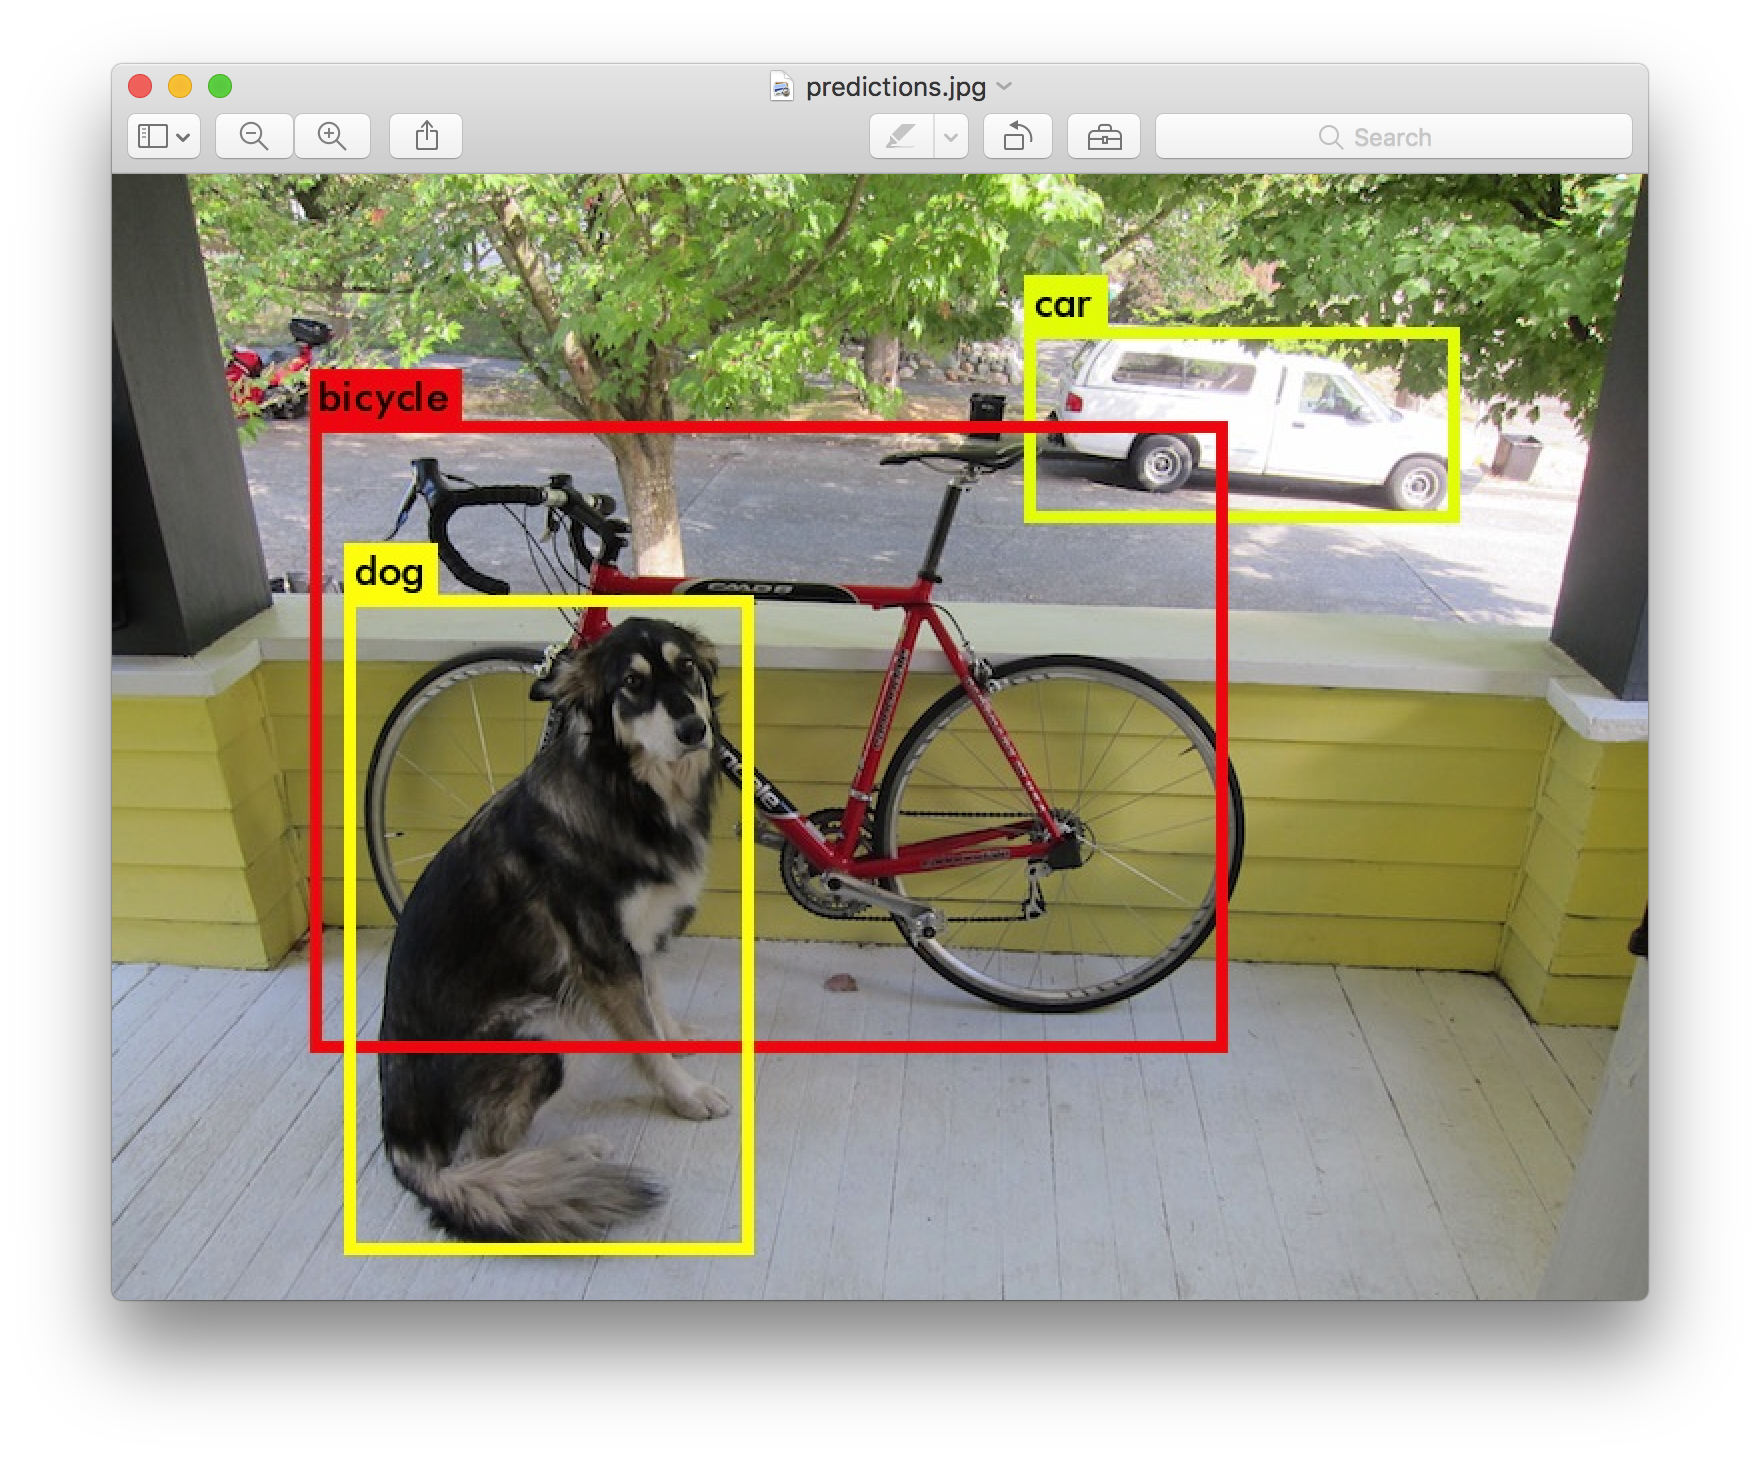
\includegraphics[scale=0.2]{ResultIMAGE.png}
\caption{탐지결과}
\label{fig:result}
\end{figure}

Darknet은 탐지한 객체와 일치도, 발견하는데 소요된 시간을 인쇄합니다.
해당 시스템은 Open CV를 이용해 컴파일하지 않았기 떄문에 탐지를 직접적으로 표시할 수 없습니다. 그렇기에 탐지된 내용을 predictions.png로 저장하고 사용자는 저장된 파일을 열어 탐지된 객체를 확인하는 방식을 사용하고 있습니다. 
해당 시스템은 CPU를 사용하기 때문에 하나의 이미지당 6초에서 12초가 소요됩니다. 
만약 GPU 환경을 사용한다면 더 빨라질 수 있습니다. 이해를 위한 몇 가지 예시 파일들을 포함시켜 놓았습니다. 확인해보시길 바랍니다. \\\\
1. data/eagle.jpg \\
2. data/dog.jpg \\
3. data/person.jpg \\
4. data/horses.jpg\\
\\
detect명령은 보다 일반적인 명령어 버전의 줄임말이며 다음 명령어와 동일합니다.

\begin{lstlisting}
 ./darknet detector test cfg/coco.data cfg/yolo.cfg yolo.weights data/dog.jpg 
\end{lstlisting}

하나의 이미지에서 탐지를 실행하는 시스템이지만 
웹캠에서 실행되는 것과 같은 다른 환경에서의 다른 작업을 수행 할 것인지를 아는 것이 유용하고
앞으로도 배우게 됩니다. 

\section{다중이미지 실습}
명령창에 이미지를 제공하는 대신 하나의 행에 여러 이미지를 시도해 볼 수 있으며 구성과 가중치가 완료되면 프롬포트가 표시됩니다.
\begin{lstlisting}
  ./darknet detect cfg/yolo.cfg yolo.weights 
  layer filters size input output 
  0 conv 32 3 x 3 / 1 416 x 416 x 3 -> 416 x 416 x 32 
  1 max 2 x 2 / 2 416 x 416 x 32 -> 208 x 208 x 32 
  ....... 
  29 conv 425 1 x 1 / 1 13 x 13 x1024 -> 13 x 13 x 425 
  30 detection 
  Loading weights from yolo.weights ...Done! 
  Enter Image Path: 
\end{lstlisting}
data/horses.jpg이미지의 경로를 입력하면 해당 이미지의 경계 영역을 예측하게 됩니다.
\begin{figure}[h!]
\centering
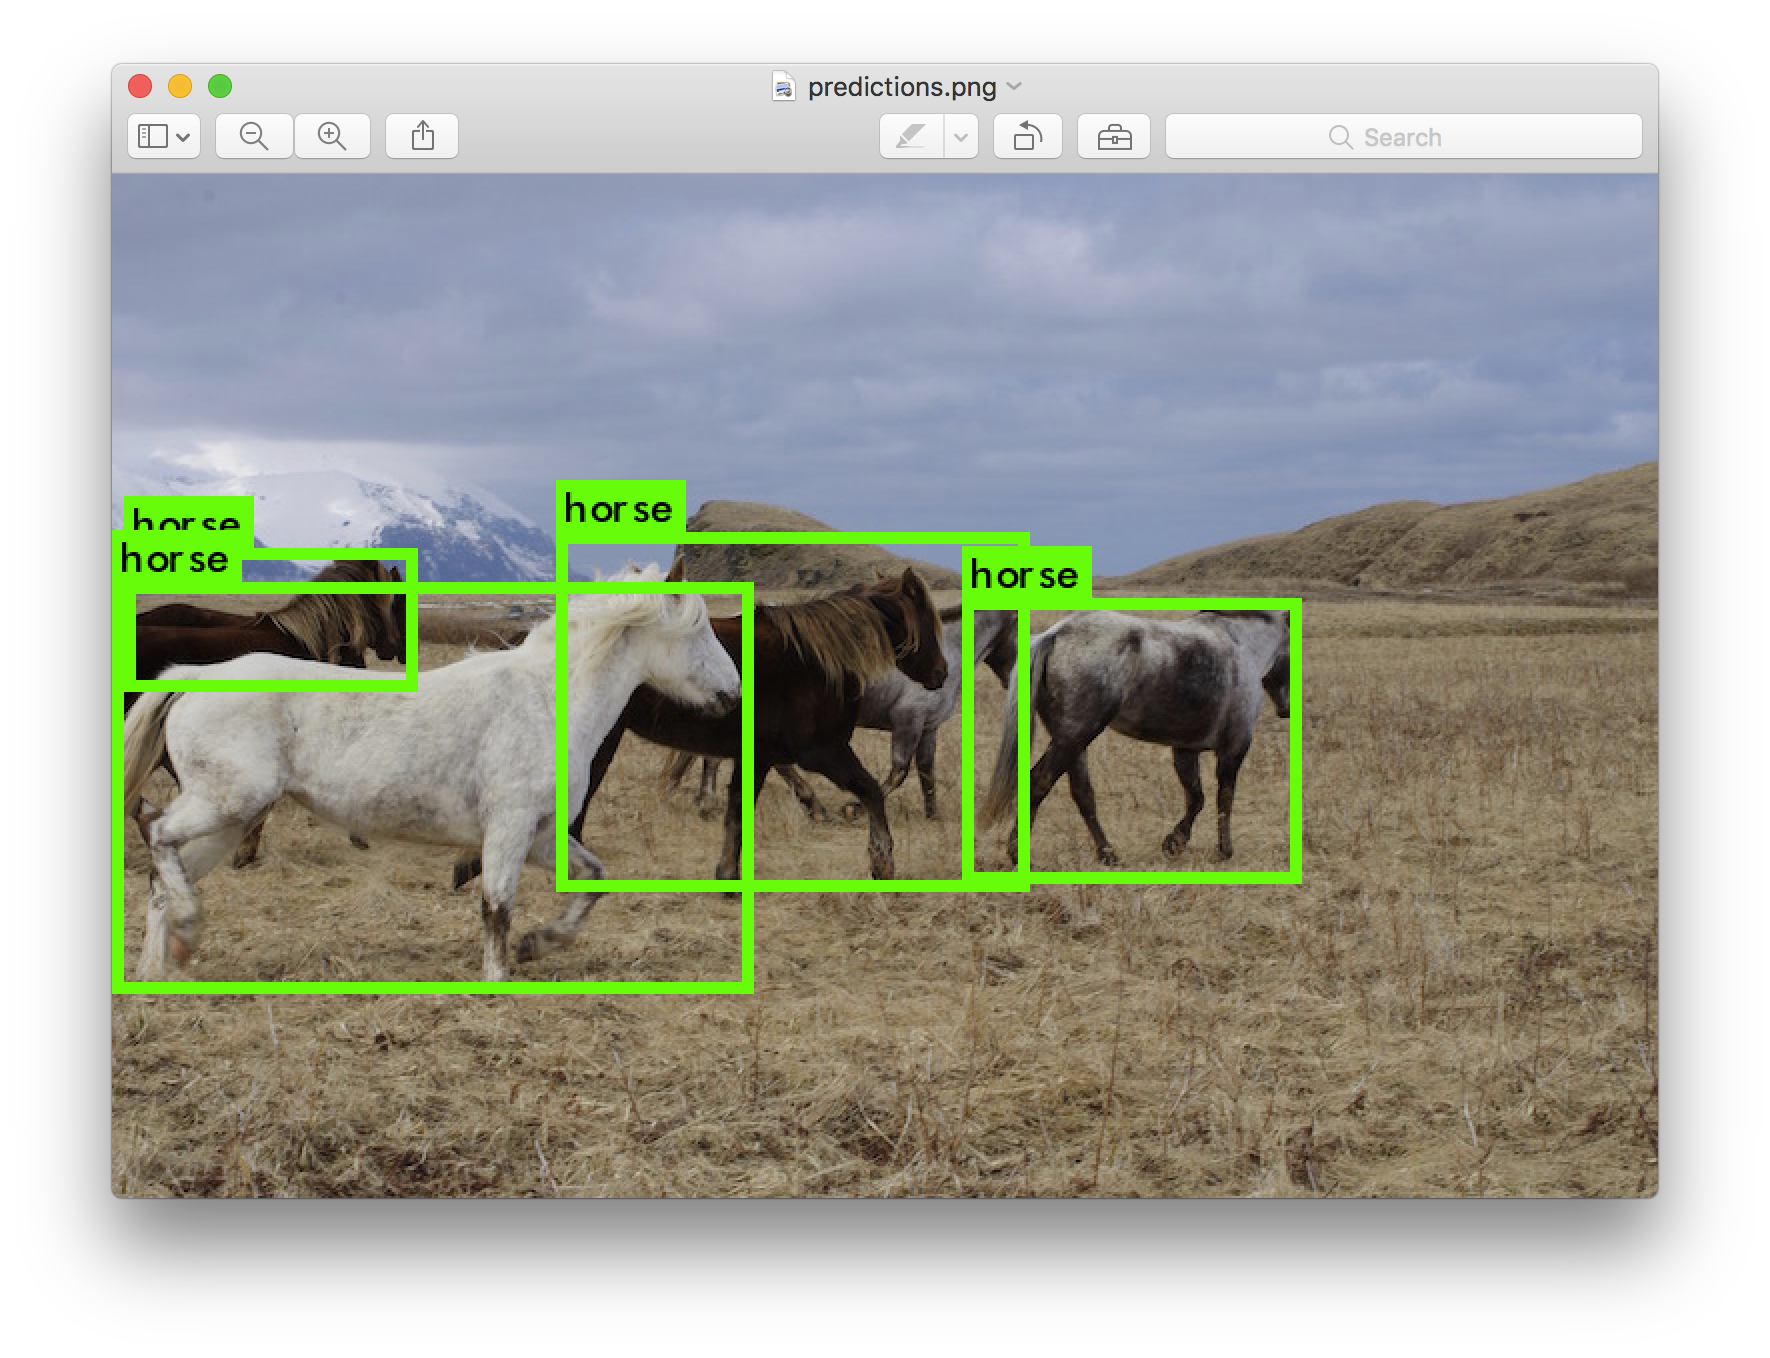
\includegraphics[scale=0.2]{horse.png}
\caption{탐지 결과}
\label{fig:horseresult}
\end{figure}
하나의 이미지가 완료되면 다른 이미지를 시도하귀 위해 더 많은 경로를 물어볼 것입니다.
Ctrl-C를 사용해 프로그램을 종료하시면 됩니다.
\section{탐색의 임계값 변경}
YOLO 시스템의 신뢰도는 기본값이 0.25이며 객체의 탐색 일치도가 0.25 이상인 객체만을 표시하여 사용자에게 보여줍니다.
이러한 임계값은 -thresh \textlangle val\textrangle 명령어 플래그를 이용하여 임계값을 변경 할 수 있습니다. 
아래의 예시는 탐색된 모든 객체를 표시하기 위하여 임계값을 0으로 설정한 것입니다. 예시 이미지를 참고하시기 바랍니다.
\begin{lstlisting}
 ./darknet detect cfg/yolo.cfg yolo.weights data/dog.jpg -thresh 0 
\end{lstlisting}
\begin{figure}[h!]
\centering
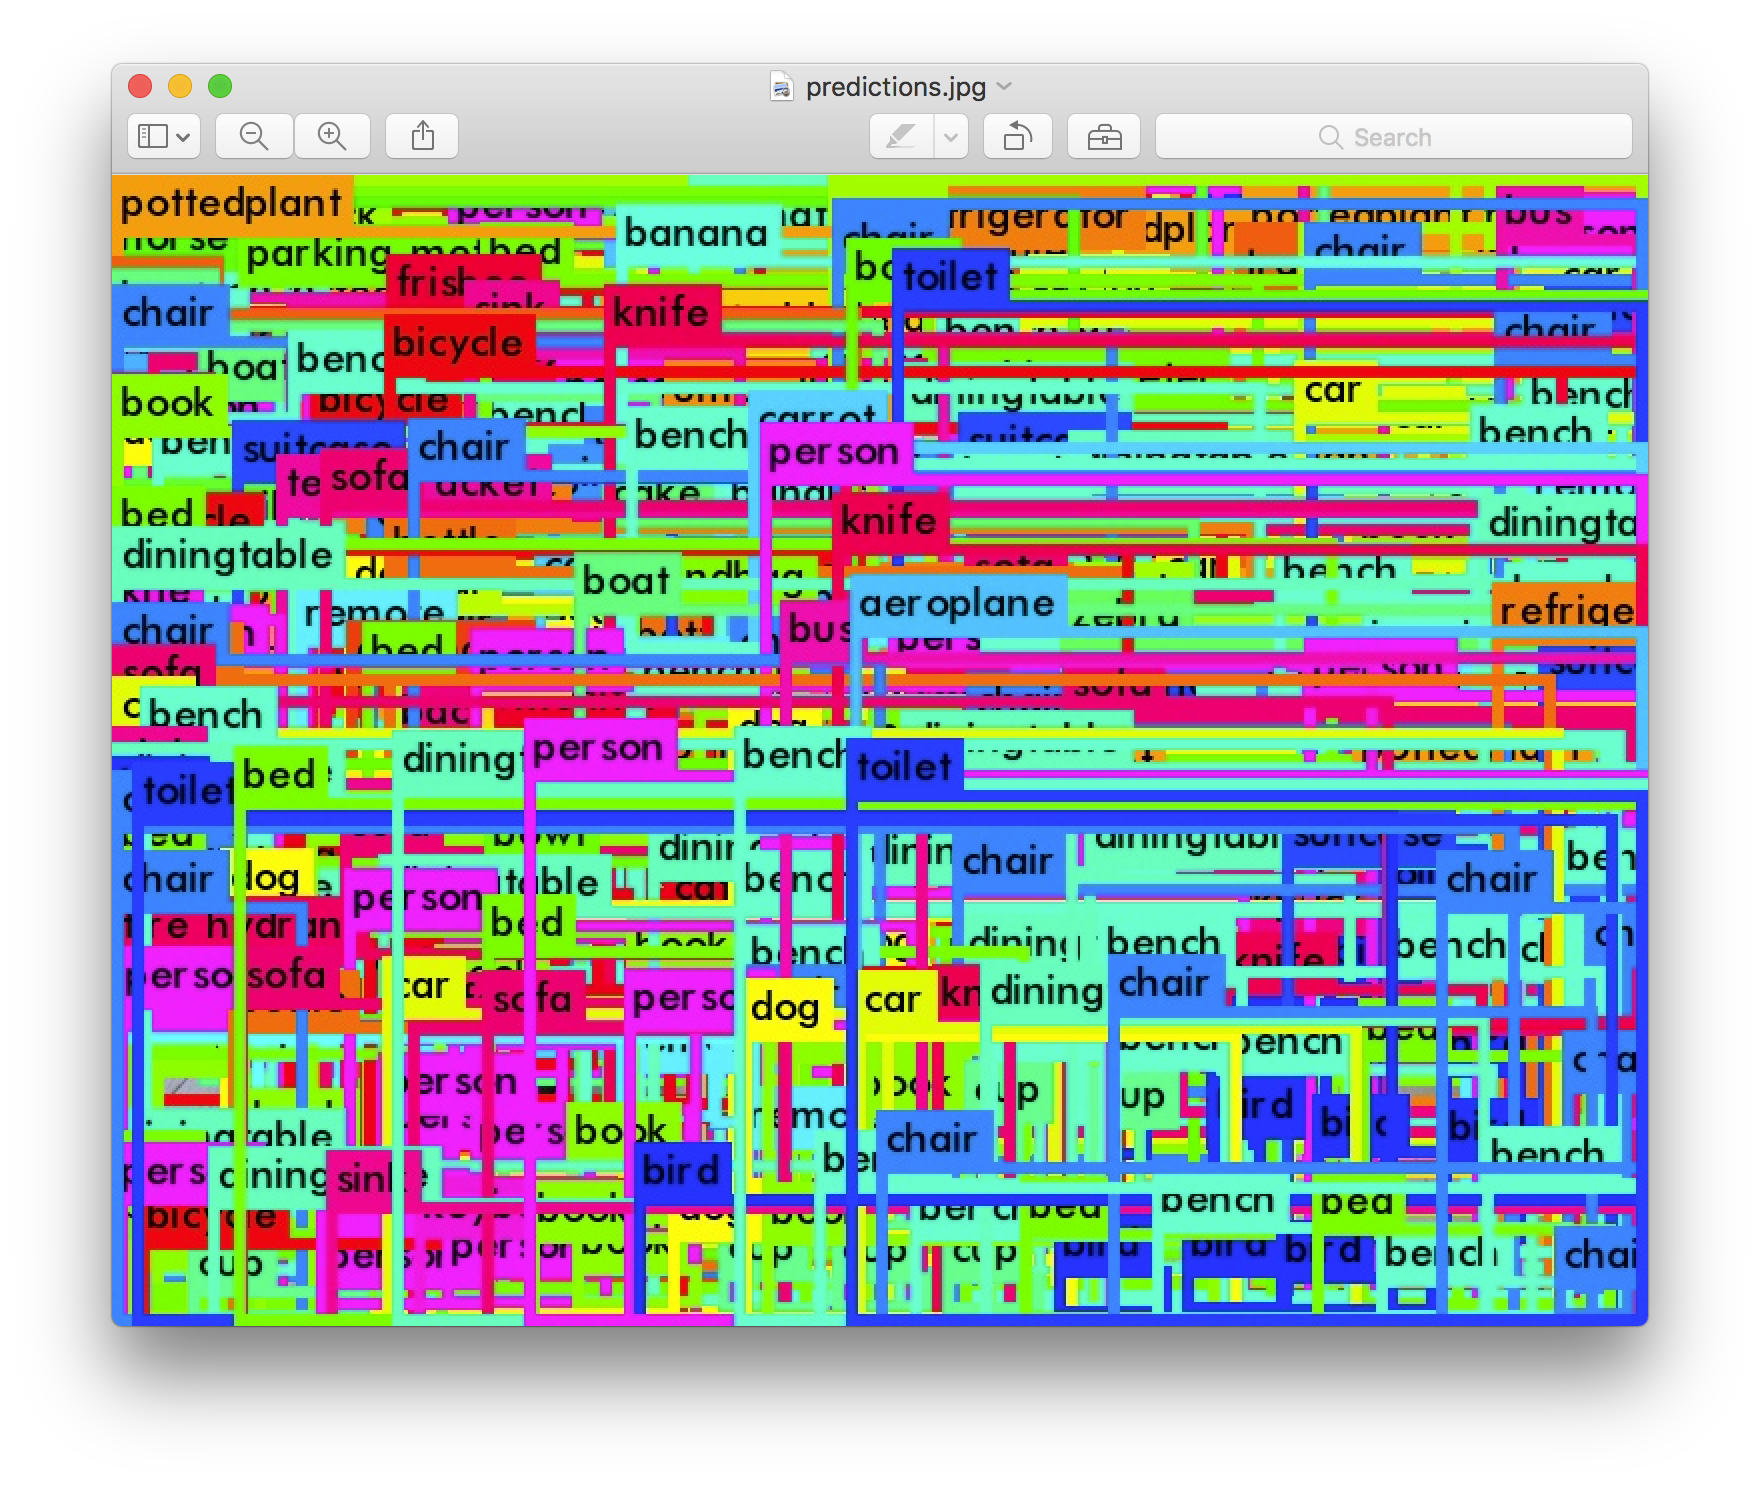
\includegraphics[scale=0.2]{eximage.png}
\caption{임계값 0 탐색결과 }
\label{fig:eximg}
\end{figure}

모델별로 임계값을 제어하는 값을 다른 값으로 설정할 수 있습니다. 
그러나 이것이 유용하다고 명백하게 말하기는 힘듭니다.

\section{TINY YOLO}
Tiny YOLO 시스템은 \href{http://khseob0715.dothome.co.kr/YOLO/reference.html}{Darknet reference network}를 기반으로 작동하며 일반 YOLO모델보다 훨씬 빠르지만 정확성이 떨어집니다.
VOC에 대한 교육 버전을 사용하려면 다음을 수행하시기 바랍니다.
\begin{lstlisting}
 wget https://pjreddie.com/media/files/tiny-yolo-voc.weights 
 ./darknet detector test cfg/voc.data cfg/tiny-yolo-voc.cfg 
                                             tiny-yolo-voc.weights data/dog.jpg 
\end{lstlisting}

어느 것이 좋고 완벽하다고 자신할 수 없지만 Tiny YOLO 시스템은 확실히 빠릅니다. 
GPU에서는 200 FPS 이상에서 실행이됩니다.
\begin{figure}[h!]
\centering
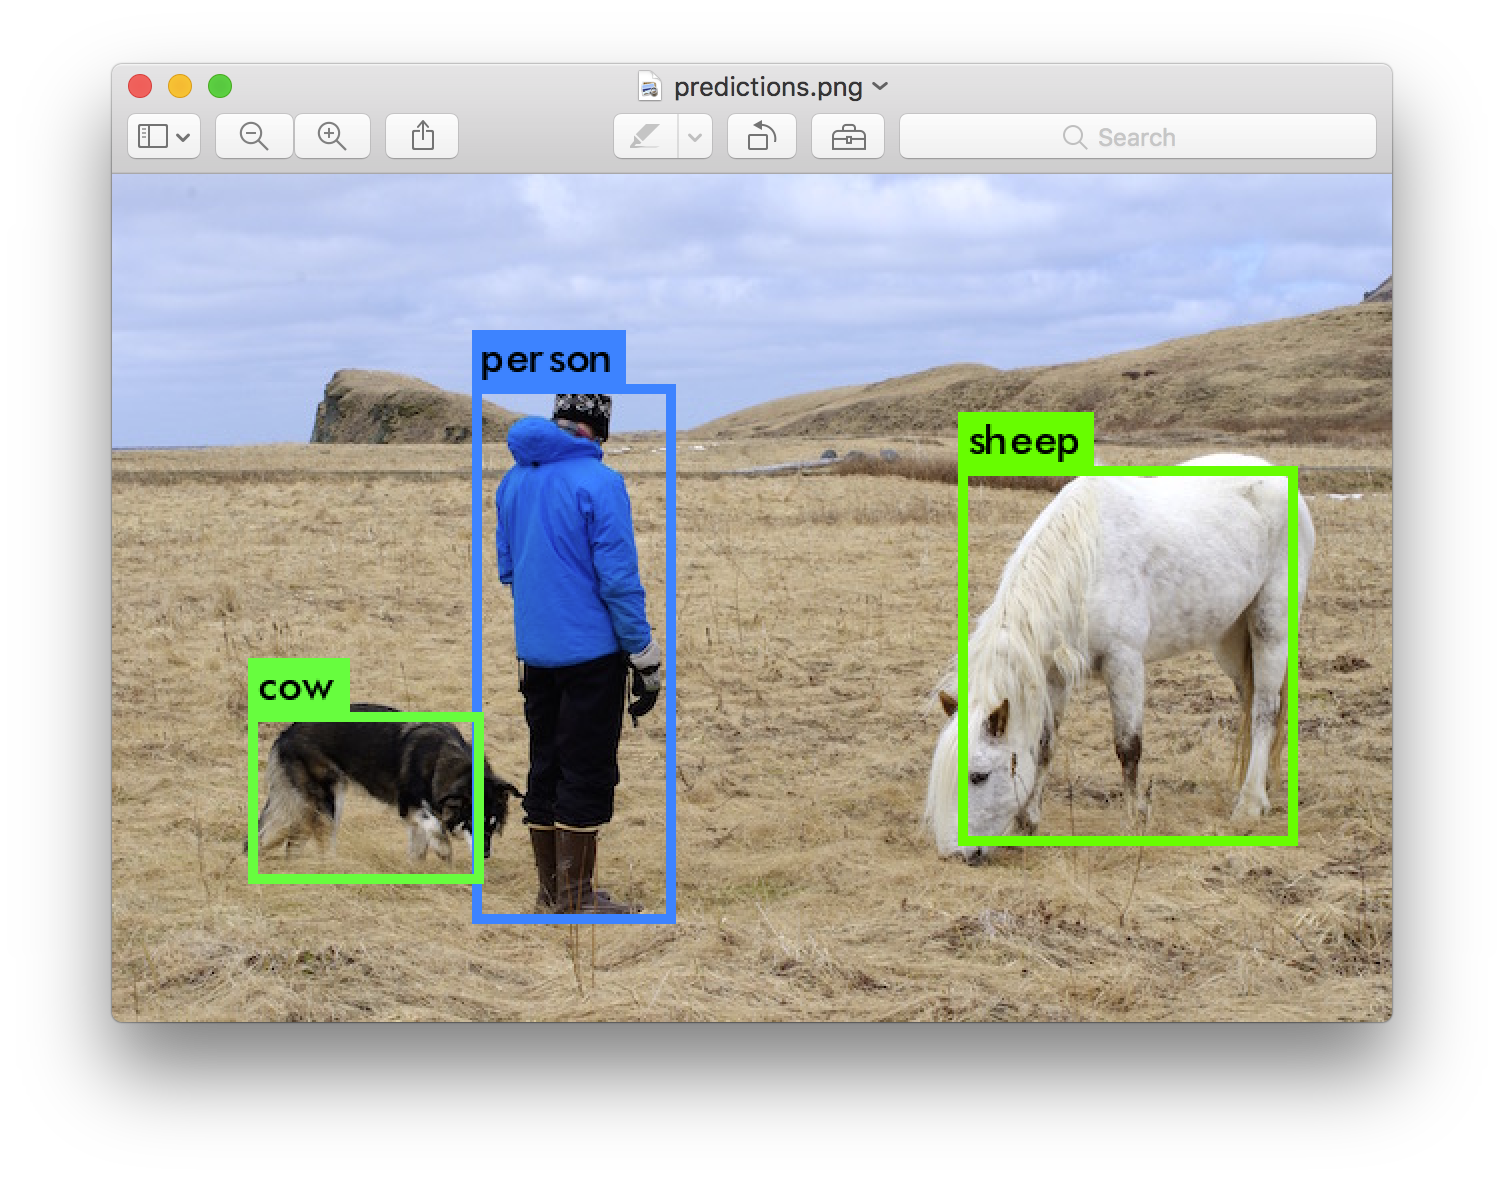
\includegraphics[scale=0.15]{tinyyolo.png}
\caption{임계값 0 탐색결과 }
\label{fig:tinyimg}
\end{figure}

\section{WEBCAM에서의 실시간 탐지}

테스트 데이터에서 YOLO 시스템을 실행하면 결과를 볼 수 없어 흥미롭지 않습니다. 
막대한 이미지 대신 웹캠의 입력으로 실행해 볼 수 있습니다.
Darkent은 CUDA와 OpenCV를 함께 사용하며 이 데모 실행을 위한 컴파일을 해야됩니다. 
다음 명령어를 실행하시기 바랍니다.
\begin{lstlisting}
 ./darknet detector demo cfg/coco.data cfg/yolo.cfg yolo.weights  
\end{lstlisting}
YOLO 시스템은 현재 FPS 및 예상 클래스뿐만 아니라 임계영역이 그려진 이미지를 표시합니다.
OpenCV가 연결할 수있는 컴퓨터에 웹캠이 연결되어 있어야합니다. 그렇지 않으면 작동하지 않습니다. 
여러 웹캠이 연결되어 있고 사용할 웹캠을 선택하려는 경우 -c \textlangle num\textrangle 입력해 플래그를 전달할 수 있습니다. 
(OpenCV가 사용하는 웹캠의 기본값은 0입니다.) OpenCV가 비디오를 읽을 수 있으면 비디오 파일에서도 실행할 수 있습니다

\begin{lstlisting}
 ./darknet detector demo cfg/coco.data cfg/yolo.cfg yolo.weights <video file> 
\end{lstlisting}
이것이 YOLO 시스템이 위의 YouTube 동영상을 만든 방법입니다

\section{VOC에서의 YOLO 훈련}
다른 훈련체계와 Hyper-Parameters 또는 데이터 셋으로 훈련을 하고 싶다면 YOLO를 처음부터 교육 할 수 있습니다. Pascal VOC 데이터 세트에서 작업하는 방법은 다음과 같습니다.

\section{PASCAL VOC DATA 얻어오기}
YOLO 시스템을 훈련 시키려면 2007 년부터 2012 년까지의 모든 VOC 데이터가 필요합니다. 
여기에서 데이터에 대한  \href{http://khseob0715.dothome.co.kr/YOLO/here.html}{링크}를 찾을 수 있습니다. 
모든 데이터를 가져 오려면 모든 디렉토리를 저장하고 해당 디렉토리에서 다음을 실행하시기 바랍니다.
\begin{lstlisting}
  wget https://pjreddie.com/media/files/VOCtrainval_11-May-2012.tar 
  wget https://pjreddie.com/media/files/VOCtrainval_06-Nov-2007.tar 
  wget https://pjreddie.com/media/files/VOCtest_06-Nov-2007.tar 
  tar xf VOCtrainval_11-May-2012.tar 
  tar xf VOCtrainval_06-Nov-2007.tar 
  tar xf VOCtest_06-Nov-2007.tar 
\end{lstlisting}
이제 VOCdevkit/ 하위 디렉토리에 모든 VOC 교육 데이터가 포함되어 있습니다.

\section{VOC에 대한 LABEL 생성}
이제 Darknet이 사용하는 레이블 파일을 생성해야합니다. 
Darknet.txt file with a line for each ground truth object in the image that looks like을 원합니다.
\begin{lstlisting}
  <object-class> <x> <y> <width> <height> 
\end{lstlisting}

여기서 x, y, width, and height 는 이미지의 높이와 너비를 기준으로. 이 파일을 생성하기 위해서
voc label.py Darknet의 스크립트 안에 scripts/ 디렉토리에 있습니다.
그냥 다시 다운로드하는게 안귀찮고 편합니다.
Darknet.txt with a line for each ground truth object in the image that looks like을 원합니다.
\begin{lstlisting}
 wget https://pjreddie.com/media/files/voc_label.py 
 python voc_label.py 
\end{lstlisting}
몇 분 후에이 스크립트는 필요한 모든 파일을 생성합니다. 대부분의 많은 파일 라벨들이 VOCdevkit/VOC2007/labels/ 그리고 VOCdevkit/VOC2012/labels/. 당신의 디렉토리에 가지고 있습니다.
\begin{lstlisting}
 ls 
 2007_test.txt VOCdevkit 
 2007_train.txt voc_label.py 
 2007_val.txt VOCtest_06-Nov-2007.tar 
 2012_train.txt VOCtrainval_06-Nov-2007.tar 
 2012_val.txt VOCtrainval_11-May-2012.tar 
\end{lstlisting}
The text files like 2007 train.txt 와 같은 텍스트 파일은 해당 연도의 이미지 파일과 이미지 세트를 나열합니다. 
DarkNet은 당신이 훈련시키고자 하는 모든 이미지를 가진 하나의 텍스트 파일을 필요로합니다. 이 예제에서
우리 모델을 테스트 할 수 있도록 2007 테스트 세트를 제외한 모든 것을 훈련시켜 봅시다
\begin{lstlisting}
 cat 2007_train.txt 2007_val.txt 2012_*.txt > train.txt 
\end{lstlisting}

이제 우리는 모든 2007 년형 trainval 과 2012 년형 trainval을 하나의 큰 목록에 포함 시켰습니다. 그것이 데이터 설정을 위해해야 할 모든 것입니다!
\section{MODIFY CFG FOR PASCAL DATA}
이제 Darknet 디렉토리로 가십시오. 데이터를 가리 키도록 cfg/voc.data구성 파일을 변경해야합니다.
\begin{lstlisting}
 1 classes= 20 
 2 train = <path-to-voc>/train.txt 
 3 valid = <path-to-voc>2007_test.txt 
 4 names = data/voc.names 
 5 backup = backup 
\end{lstlisting}
\textlangle path-to-voc\textrangle 을 VOC 데이터를 저장 한 디렉토리로 대체해야합니다.
\section{사전 훈련된 CONVOLUTIONAL 가중치 다운로드}
교육을 위해 우리는 Imagenet에서 사전 훈련 된 Extraction model의 가중치를 사용합니다.
레이어 가중치 다운로드 
\begin{lstlisting}
 wget https://pjreddie.com/media/files/darknet19_448.conv.23 
\end{lstlisting}
사전 훈련 된 가중치를 직접 생성하려면 사전 교육 된 Darknet19 448x448 model 의 다음 명령을 실행하십시오.
\begin{lstlisting}
 ./darknet partial cfg/darknet19_448.cfg darknet19_448.weights 
                                                      darknet19_448.conv.23 23 
\end{lstlisting}
하지만 가중치 파일을 다운로드하면 더 쉽게 사용할 수 있습니다.
\section{모델 훈련}
아래의 명령어를 이용해 훈련을 시킬 수 있습니다.
\begin{lstlisting}
 ./darknet detector train cfg/voc.data cfg/yolo-voc.cfg 
                                                      darknet19_448.conv.23 
\end{lstlisting}

\section{COCO에서의 YOLO 훈련}
만약 다른 훈련체계, Hyper-Parameters 또는 데이터셋을 사용하고 싶다면 YOLO를 처음부터 훈련 시킬 수 있습니다. 
\href{http://cocodataset.org}{COCO 데이터셋}에서 작업을 하는 방법은 다음과 같습니다.

\section{COCO DATA 얻어오기}
YOLO 시스템을 훈련시키기 위해서는 모든 COCO의 데이터와 라벨이 필요합니다. 
scripts/get coco dataset.sh 이 스크립트가 해당 작업을 수행합니다. 
COCO 데이터를 넣고 다운로드 하려면 아래를 참고하시면 됩니다.
\begin{lstlisting}
 cp scripts/get_coco_dataset.sh data 
 cd data 
 bash get_coco_dataset.sh 
\end{lstlisting}
이제 Darknet에 모든 데이터와 라벨을 생성해야 합니다.

\section{COCO의 CFG 수정}
이제 Darknet 폴더로 이동합니다. 
cfg/coco.data를 가리키도록 config 파일을 변경해야 합니다.
\begin{lstlisting}
  1 classes= 80 
  2 train = <path-to-coco>/trainvalno5k.txt 
  3 valid = <path-to-coco>/5k.txt 
  4 names = data/coco.names 
  5 backup = backup 
\end{lstlisting}
COCO 데이터를 저장하는 디렉토리로 <path-to-coco>를 대체해야합니다.
또한 cfg를 테스팅 용이 아닌 훈련용으로 수정해야합니다. 
cfg/yolo.cfg가 아래와 같아야 합니다.
\begin{lstlisting}
  [net] 
  # Testing 
  # batch=1 
  # subdivisions=1 
  # Training 
  batch=64 
  subdivisions=8 
  .... 
\end{lstlisting}
\section{모델 훈련}
이제부터 모델 훈련을 위해 아래 명령어를 실행하시기 바랍니다.
\begin{lstlisting}
 ./darknet detector train cfg/coco.data cfg/yolo.cfg 
                                              darknet19_448.conv.23 
\end{lstlisting}
만약 여러개의 GPU를 사용한다면 다음 명령어를 실행하시기 바랍니다.
\begin{lstlisting}
 ./darknet detector train cfg/coco.data cfg/yolo.cfg 
                                              darknet19_448.conv.23 -gpus 0,1,2,3 
\end{lstlisting}
만약 Checkpoint에서 훈련을 중지하고 다시 시작하기 위해서는 다음 명령어를 실행하시기 바랍니다.
\begin{lstlisting}
 ./darknet detector train cfg/coco.data cfg/yolo.cfg 
                                              backup/yolo.backup -gpus 0,1,2,3
\end{lstlisting}


\section{DARKNET 설치 방법}
Darknet은 다음과 같이 두가지 방식을 사용하면 설치하기 쉽습니다.

\begin{verbatim}
OpenCV:다양하게 지원되는 이미지 유형을 원할 경우  
CUDA:CPU계산을 원할 경우
\end{verbatim} 
둘 다 선택 사항이므로 기본 시스템을 설치하는 것만으로 시작할 수 있으며 테스트 환경은 리눅스와 맥 환경에서만 실시하였습니다.

\section{기본 시스템 설치}
\begin{verbatim}
기본 시스템을 설치합니다. 
\end{verbatim}
Darknet git 저장소를  다운하시기 바랍니다. 다음 명령어들을 참고하시면 됩니다.
\begin{verbatim}
1. git clone https://github.com/pjreddie/darknet.git 
2. cd darknet 
3. make 
\end{verbatim}
이러한 작업을 수행하면 다음과 같은 많은 정보를 수집해야합니다.
\begin{verbatim}
1. gcc -I/usr/local/cuda/include/ -Wall -Wfatal-errors -Ofast.... 
2. gcc -I/usr/local/cuda/include/ -Wall -Wfatal-errors -Ofast.... 
3. gcc -I/usr/local/cuda/include/ -Wall -Wfatal-errors -Ofast.... 
   .... 
n. gcc -I/usr/local/cuda/include/ -Wall -Wfatal-errors -Ofast -lm.... 
\end{verbatim}
모든 수집 정보들을 모은 것이 확인됬다면 프로그램을 실행하시기 바랍니다.

\begin{verbatim}
  ./darknet 
\end{verbatim}
다음과 같은 출력 결과를 얻어야합니다.
\begin{verbatim}
 usage: ./darknet <function>

\end{verbatim}
얻어졋다면 이제 \href{https://pjreddie.com/darknet/}{여기서} 여러분이 
할 수 있는 일들을 확인하시기 바랍니다.

\section{CUDA와 협업}

\begin{verbatim}
  ./darknet 
\end{verbatim}
CPU에 있는 Darknet은 빠르지만 GPU에서 500배 더 빠릅니다! 그러기에  \href{https://developer.nvidia.com/cuda-gpus}{Nvidia GPU} 와 \href{https://developer.nvidia.com/cuda-downloads}{CUDA} 설치해야 합니다. 
CUDA 설치에 관해서는 복잡한 내용이기에 깊게 다루지는 않겠습니다.

\begin{verbatim}
CUDA가 설치되어 있다면 기본 디렉토리에서 Makefile의 첫번째 행을 읽기 전용으로 바꿔줍니다.
\end{verbatim}
 GPU=1 

\begin{verbatim}
이제 여러분은 make 입력하면 프로젝트를 생성하고 CUDA를 활성화 할 수 있습니다. 
CUDA가 올바르게 설치됬다면 nvidia-smi 명령어를 이용해 당신의 그래픽 카드 리스트를 확인할 수 있으며 기본적으로 시스템의 우선 순위로 그래픽 카드를 네트워크에서 실행합니다. 
또한 당신이 Darknet을 이용하는데 그래픽 카드를 바꾸기를 원한다면
명령어 줄의 flag -i <index>를 아래를 참고하여 바꾸시면 됩니다.
\end{verbatim}
  ./darknet -i 1 imagenet test cfg/alexnet.cfg alexnet.weights 
 
\begin{verbatim}
만약 여러분이 CUDA를 사용하여 컴파일 할 수 있지만 어떤 이유로든 
사용할 수 있는 CPU계산을 위해 CPU를 대신하여-nogpu 명령어를 사용하세요.
\end{verbatim}
   ./darknet -nogpu imagenet test cfg/alexnet.cfg alexnet.weights 

\section{OPENCV를 이용한 컴파일}

\begin{verbatim}
기본적으로 Darknet은 이미지 로딩을 위해 stb_image.h 를 사용합니다. 또한 OpenCV를 사용하면 디스크에 저장하지 않아도 이미지와 탐지 기능을 볼 수 있습니다.
\end{verbatim}
우선 OpenCV를 먼저 설치하세요.
소스에서 이 작업을 수행하면 오래걸리고 복잡하므로 패키지 매니저를 사용하여 수행할 수 있습니다.

\begin{verbatim}
다음으로 Makefile의 두번째 줄을 변경합니다.
\end{verbatim}
 OPENCV=1 
 
\begin{verbatim}
다 끝났습니다! 실행하기 전, 우선 다시 make를 사용해 프로젝트를 다시 시작하세요. 그 다음 imtest 사용하여 영상 로드를 테스트하고 다음을 표시합니다.
\end{verbatim}
 ./darknet imtest data/eagle.jpg 
 
 \begin{verbatim}
지금까지의 절차대로 정상적으로 동작한다면 사진과 같이 보일 것입니다.
\end{verbatim}
\begin{figure}[h!]
\centering
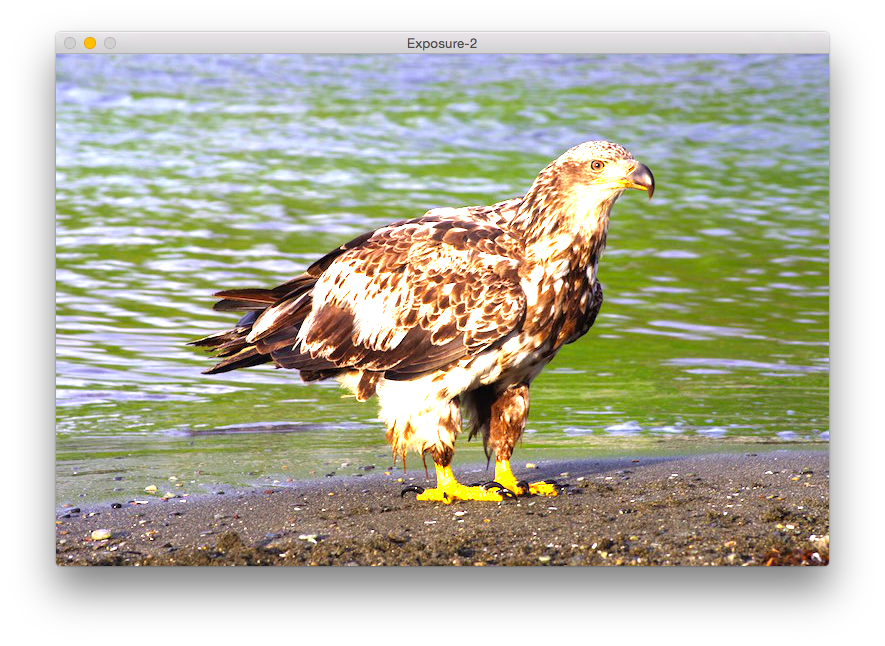
\includegraphics[scale=0.2]{egle.png}
\caption{출력 결과}
\label{fig:detect}
\end{figure}
 
  


\section{YOLO OSS 구현하기}

\author{Window 환경 }

\begin{verbatim}
YOLO OSS는 구현 기반이 Linux 기반으로 구성되어 있습니다. 따라서 Windows 환경에서는 구현내용이 다소 복잡하고 어려울수 있으나 아래내용을 따라하게 되면 누구나 쉽게 이용하실수 있습니다!

\end{verbatim}

YOLO 윈도우 버전 :: \href{https://github.com/AlexeyAB/darknet/}{https://github.com/AlexeyAB/darknet/}

첫번째 사이트(AlexeyAB)에 가면 YOLO 윈도우 버전을 다운받을 수 있습니다. 또한 설치, 컴파일, 실행 방법까지 상세하게 설명되어 있습니다. 따라서 설명만 따르면 어렵지 않게 빌드 및 테스트가 가능합니다.

순서는 다음과 같습니다.

\begin{verbatim}
1. MSVS2015, CUDA8.0, OpenCV3.0 을 이미 설치하고 있다면 

(경로설정을 C:\opencv3.0\opencv\build\include & C:\opencv3.0\opencv\build\x64\vc14\lib ) 으로 해줍니다 그후에
MSVS2015를 실행하고 build\darknet\darknet.sln 의 설정을 x64, Release 설정은 Build -> Build 로 바꾸어 줍니다.


2. C : \ opencv_3.0 \ opencv \ build \ x64 \ vc14 \ bin에있는 opencv_world320.dll
및 opencv_ffmpeg320_64.dll 파일을 찾아 darknet.exe 파일과 함께 둡니다.
\end{verbatim}



\begin{figure}[h!]
\centering
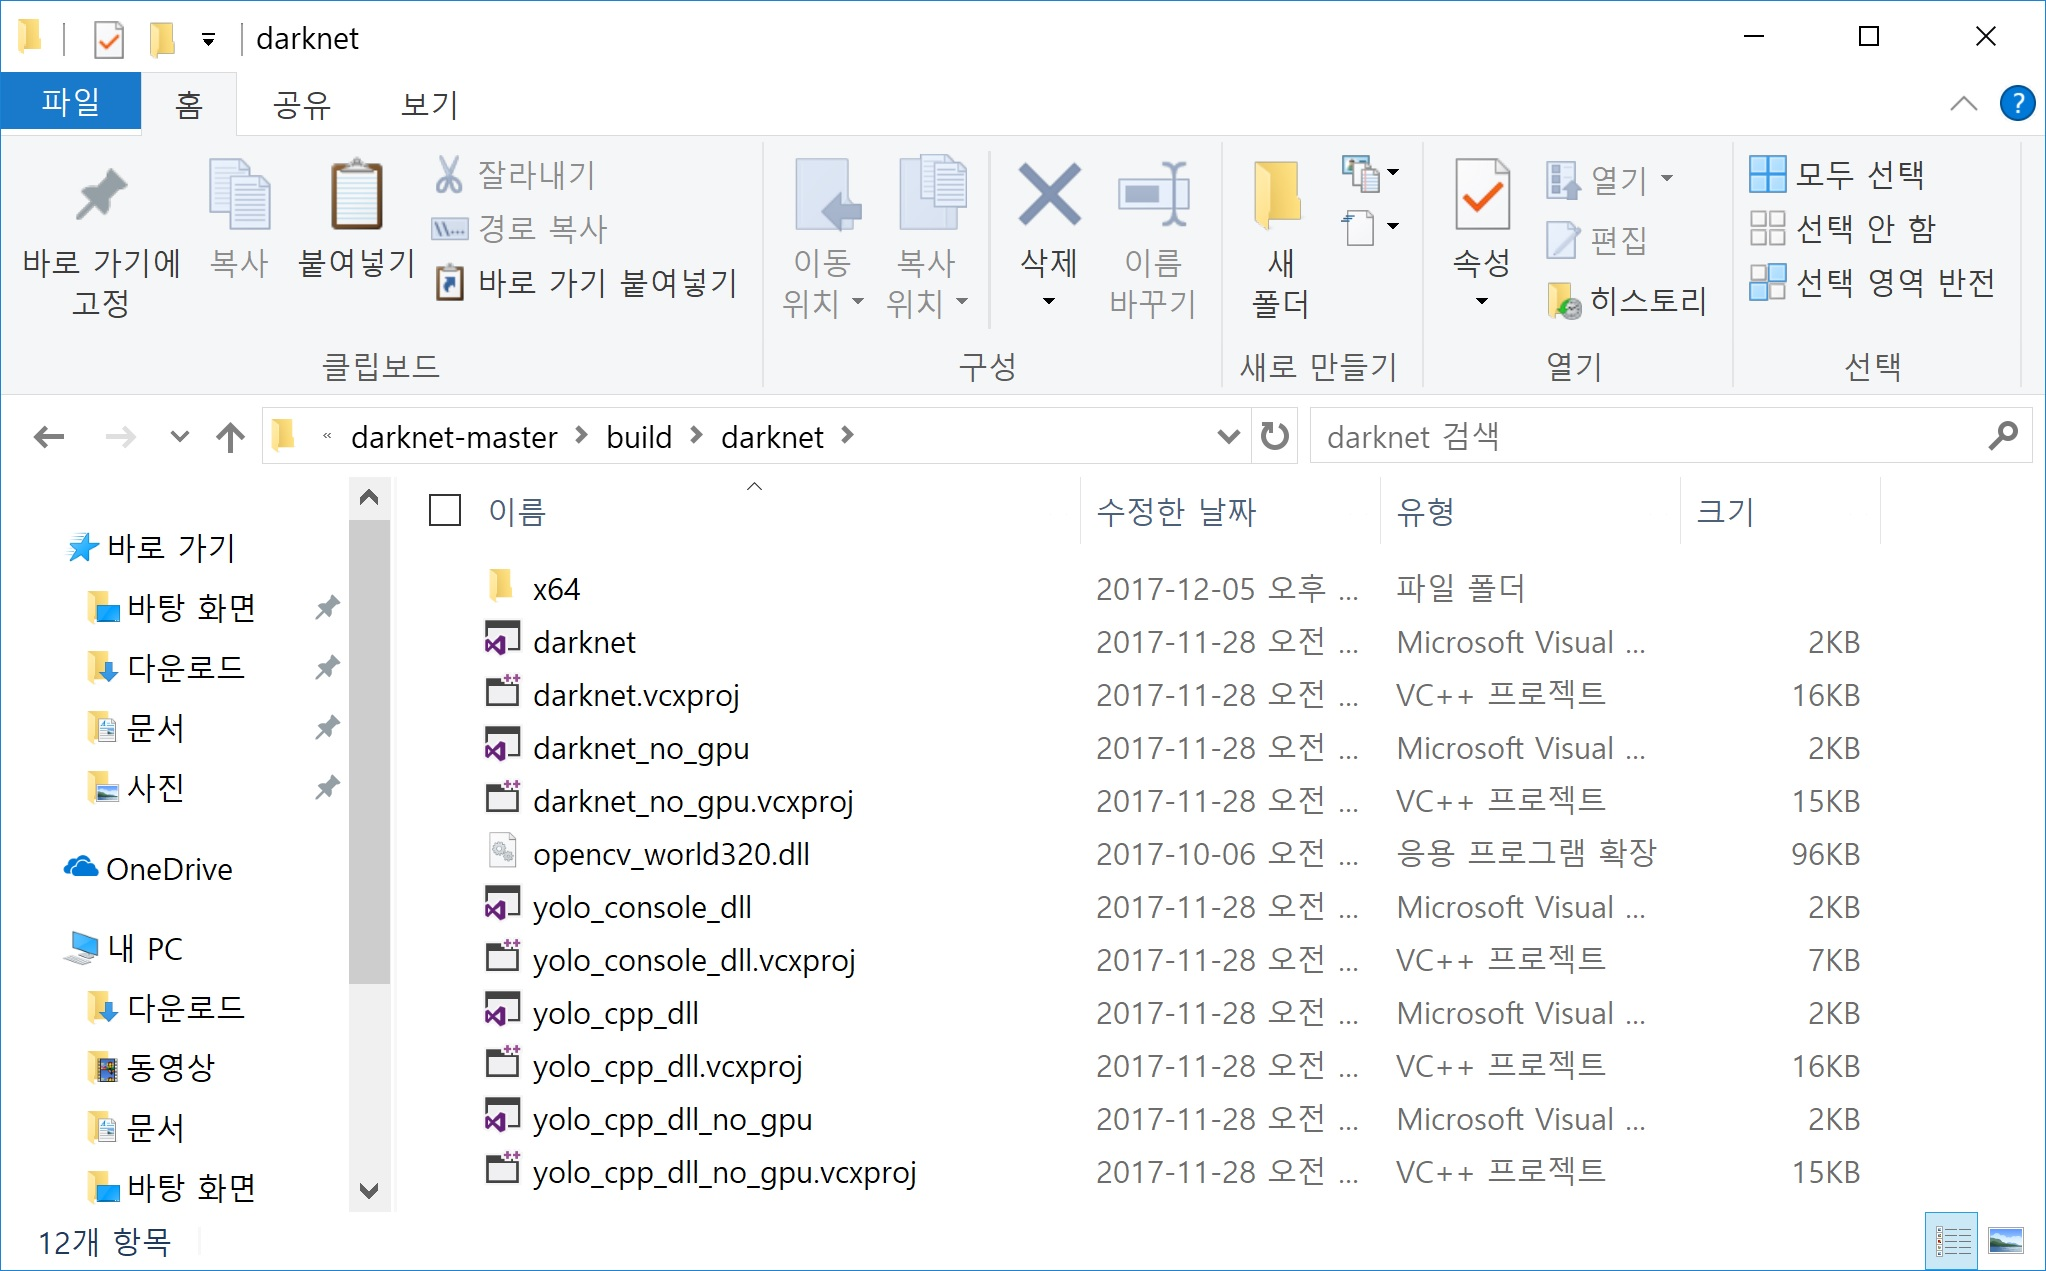
\includegraphics[scale=0.2]
{how/setting_darknet.jpg}
\caption{opencv를 이용한 setting}
\label{fig:detect}
\end{figure}

\begin{verbatim}
3. 다른 버전의 CUDA (8.0 아님)를 가지고 있다면 메모장을 사용하여 build \ darknet \ darknet.vcxproj를 열고 "CUDA 8.0"으로 2 곳을 찾아 CUDA- 버전으로 변경 한 다음 1 단계를 수행하십시오


4. MSVS 2015 및 OpenCV 3.0 (경로 : C : \ opencv_3.0 \ opencv \ build \ include 
및 C : \ opencv_3.0 \ opencv \ build \ x64 \ vc14 \ lib)
에있는 경우 MSVS를 시작하고 

build \ darknet \ darknet_no_gpu.sln을 열고 x64 및 Release를 설정하고 다음을 수행하시면됩니다.
그리고 빌드설정은 빌드 -> 빌드 darknet 로 하면 됩니다.
\end{verbatim}

\begin{figure}[h!]
\centering
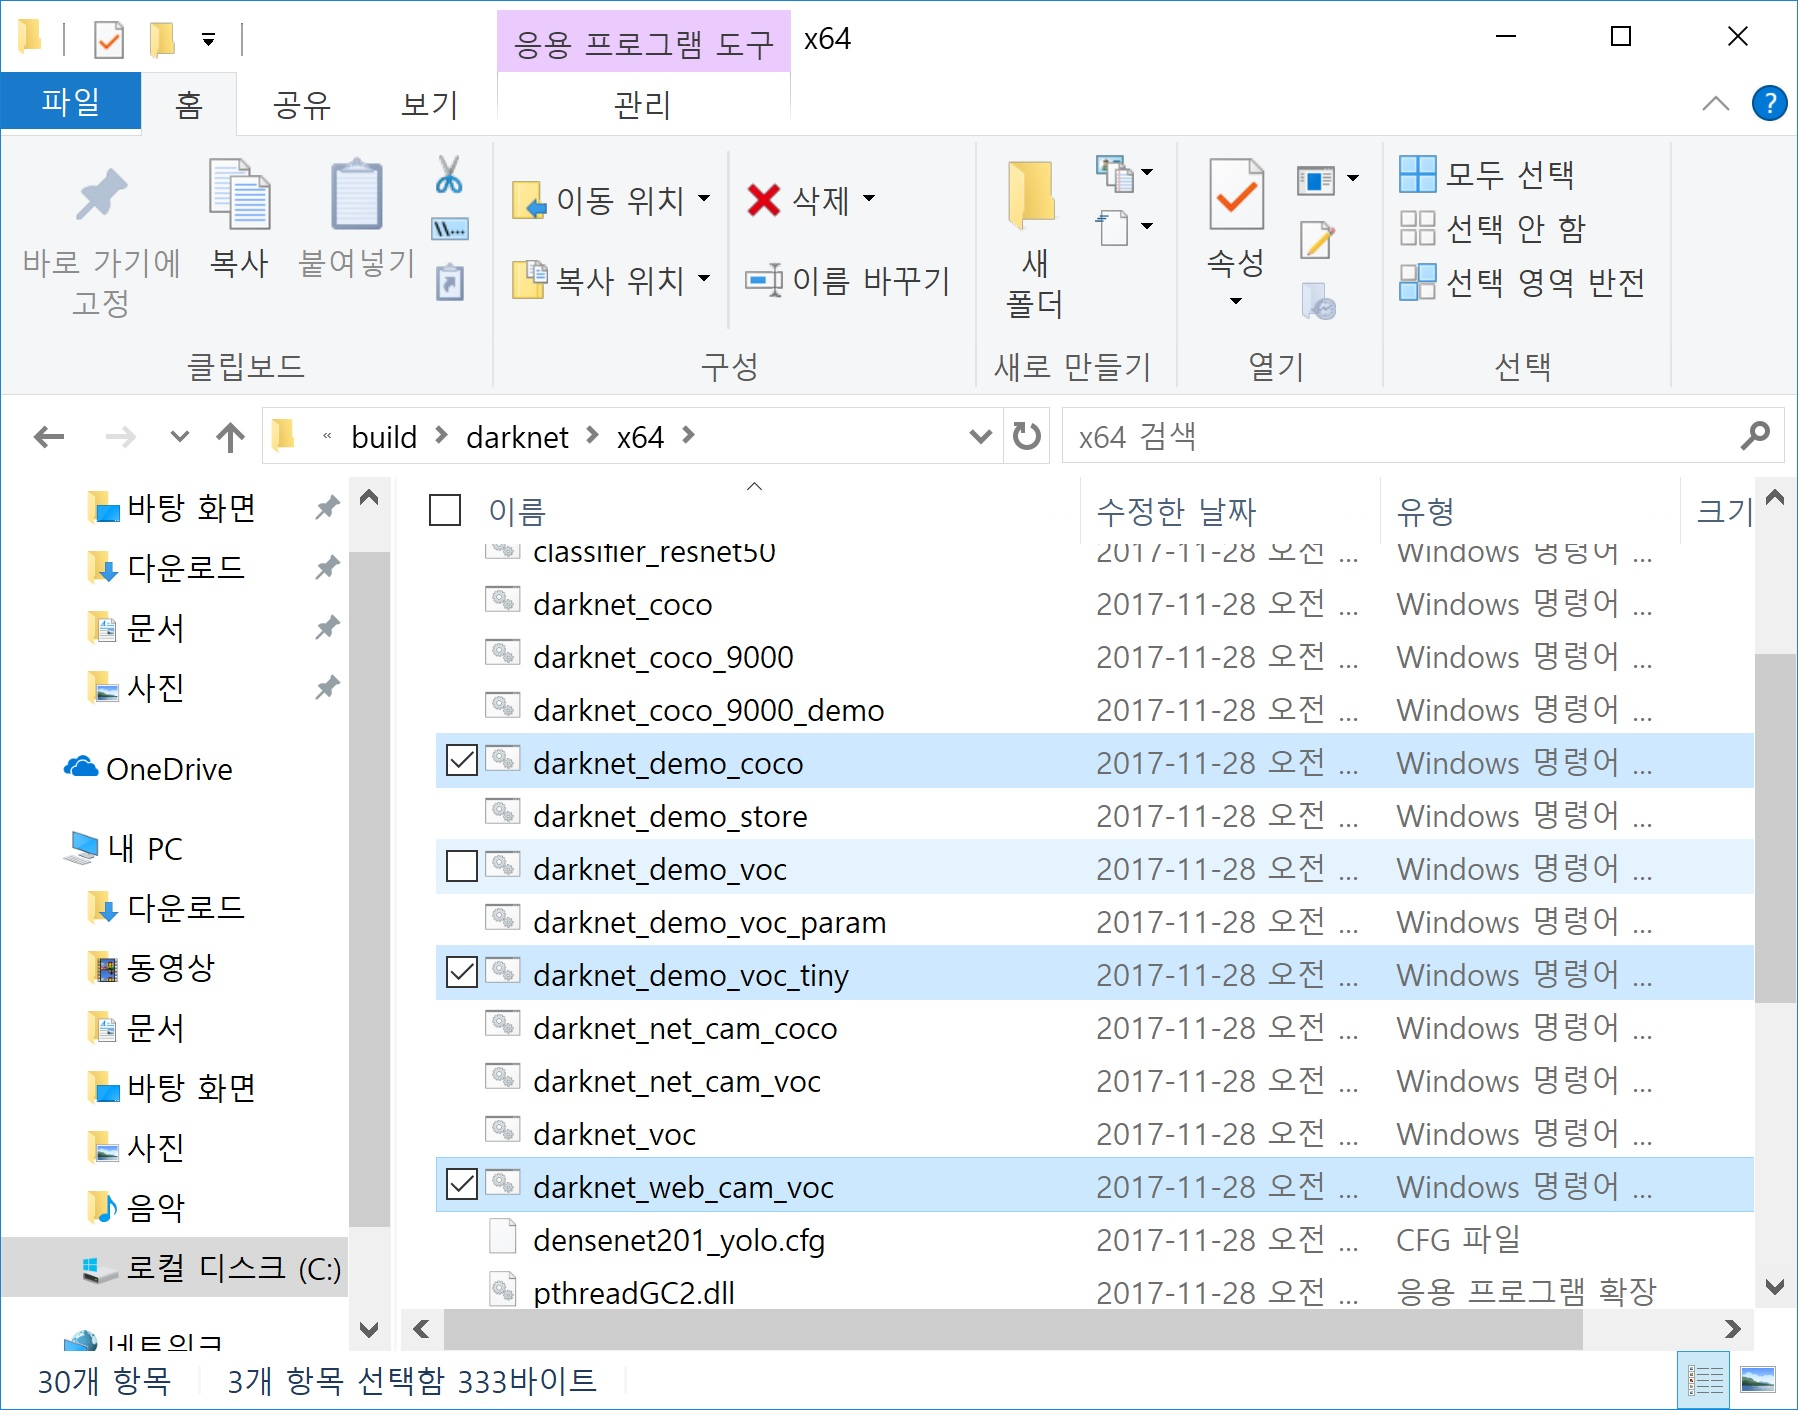
\includegraphics[scale=0.2]
{how/setting2.jpg}
\caption{opencv를 이용한 setting2}
\label{fig:detect}
\end{figure}

\begin{verbatim}
5. 3.0 대신 OpenCV 2.4.13을 사용하고 있다면 \ darknet.sln을 연 후 pathes를 변경해야합니다

- (우측클릭 속성) -> 속성(properties) -> C/C++ -> General -> Additional Include Directories:
C:\opencv_2.4.13\opencv\build\include

- (우측클릭 속성) -> 속성(properties) -> Linker -> General -> Additional Library Directories:
C:\opencv_2.4.13\opencv\build\x64\vc14\lib


6. 속도 향상을 위해 CUDNN으로 빌드하려면 다음을 수행하십시오.

-download and install cuDNN 6.0 for CUDA 8.0: https://developer.nvidia.com/cudnn

-add Windows system variable cudnn with path to CUDNN: https://hsto.org/files/
a49/3dc/fc4/a493dcfc4bd34a1295fd15e0e2e01f26.jpg

-open \darknet.sln -> (right click on project) -> properties -> C/C++ -> Preprocessor
-> Preprocessor Definitions, and add at the beginning of line: CUDNN;











\end{verbatim}

\section{YOLO OSS 구현 화면}


\begin{figure}[h!]
\centering
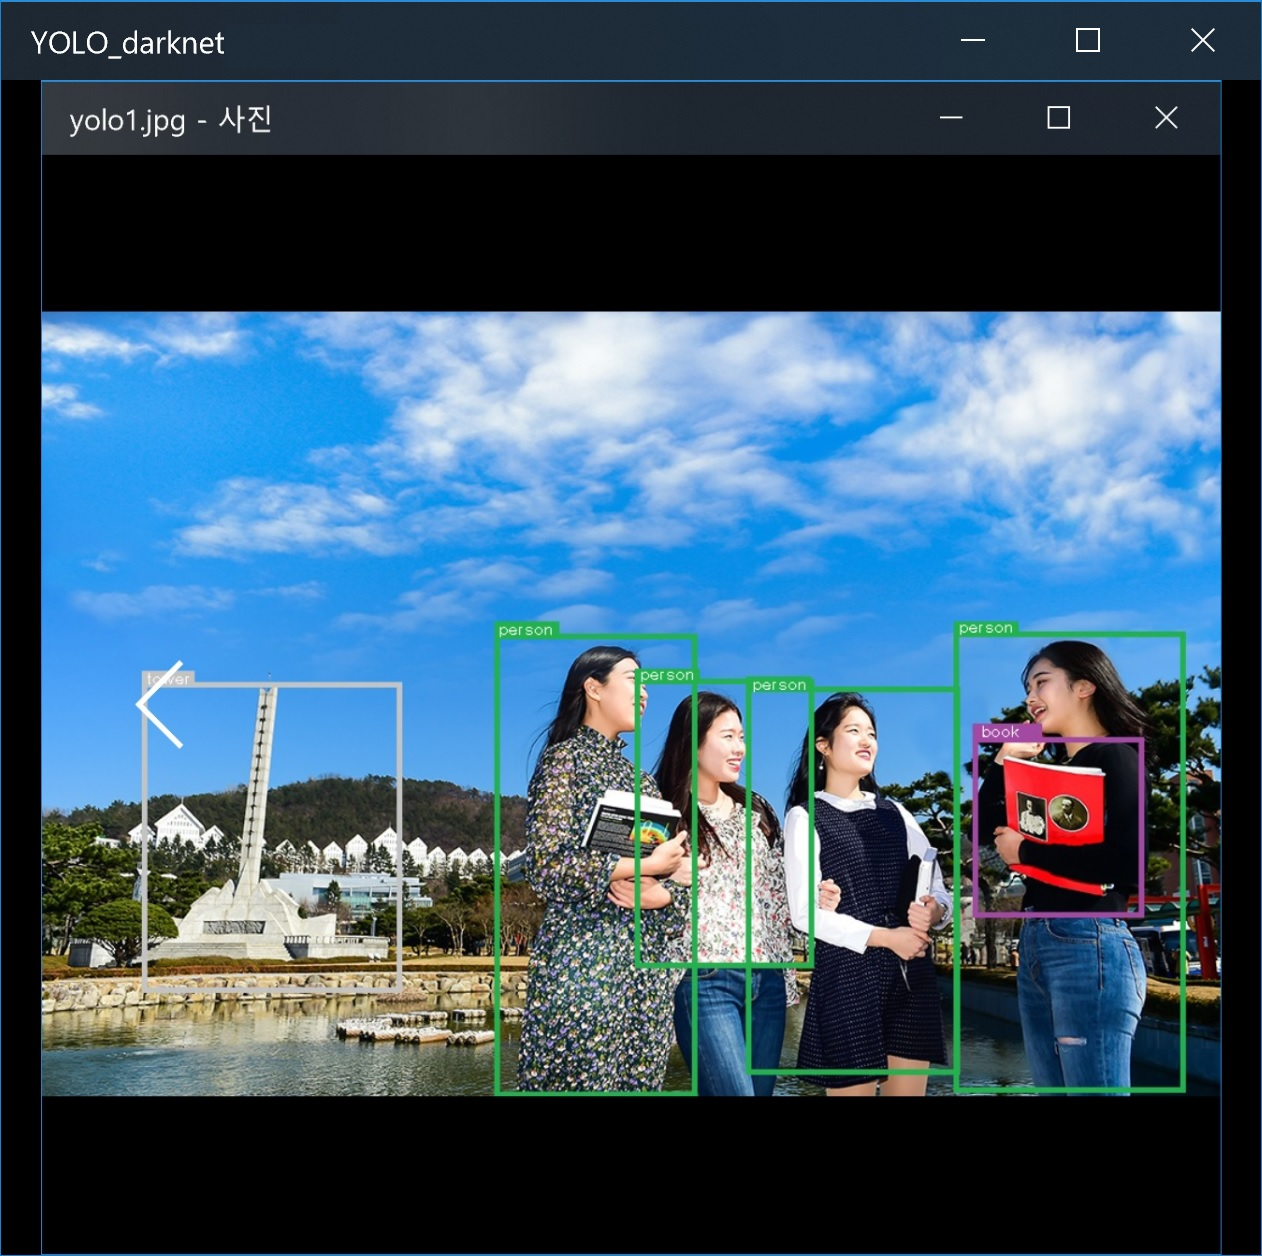
\includegraphics[scale=0.4]
{how/YOLO_darknet_1.jpg}
\caption{YOLO-darknet 구현화면 1}
\label{fig:detect}
\end{figure}

\begin{figure}[h!]
\centering
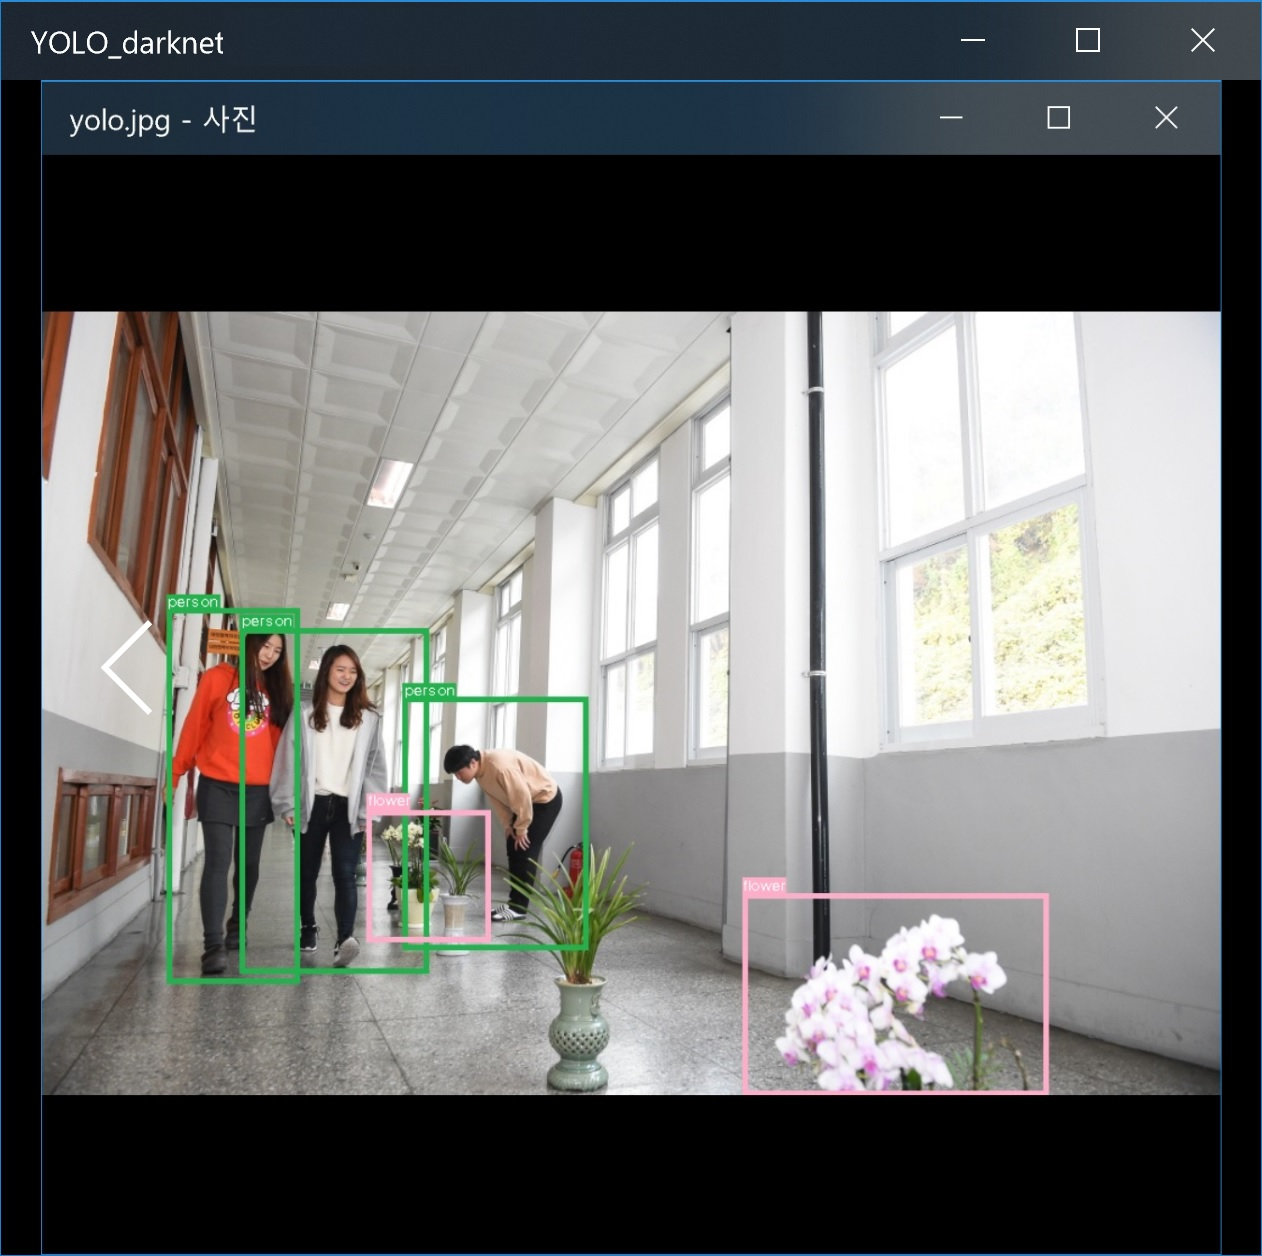
\includegraphics[scale=0.4]
{how/YOLO_darknet_.jpg}
\caption{YOLO-darknet 구현화면 2}
\label{fig:detect}
\end{figure}


\begin{verbatim}
다음 사진과 같이 학습된 데이터 셋을 통해 image 를 인식하고 해당 정보를 표시해줍니다.    

다운받은 소스에 보면 여러 가지 설정의 Visual Studio (VS) 프로젝트 파일들이 제공됩니다. 이 중에서 yolo_cpp_dll 버전으로 빌드 및 테스트를 했습니다. yolo를 dll 라이브러리로 만들어 놓으면 다른 윈도우즈 프로그램에서도 자유롭게 사용할 수 있기 때문입니다.



다만, 한 가지 문제는 사이트에서 제공하는 프로젝트 파일은 Visual Studio 2015 용이기 때문에 그 이전버전의 Visual Studio(VS 2013 등)에서는 사용이 안된다는 점이 있습니다.



한 가지 해결법은 다음과 같습니다. (1) 먼저, *.sIn 파일을 삭제한다. (2) 이후 *.vcxproj 파일을 메모장으로 열어서 프로젝트의 버전을 자신의 VS에 맞게 수정해 준다. (3) 이후 수정된 *.vcxproj를 클릭하여 프로젝트를 연다 (프로젝트를 저장하면 *.sIn 파일이 자신의 버전에 맞게 자동 생성됩니다).



예를 들어, 자신이 사용하는 버전이 Visual Studio 2013라면 14.0은 12.0으로 v140은 v120으로 변경해 주면 됩니다.

\end{verbatim}




\bibliographystyle{plain}
\bibliography{references}


\end{document}


